\documentclass{beamer}
\usepackage[T1]{fontenc}
\usepackage{lmodern}
\usepackage{graphicx}
\usepackage{amsmath}
\usepackage{amsbsy}
\usepackage{amssymb}
\usepackage{bm}
\usepackage{calc} 
\usepackage{tikz}                                       
\usetikzlibrary{positioning,graphs,calc,backgrounds,fit,patterns}

\mode<presentation>
\usetheme[footline=empty]{Magicc}

\global\long\def\x{\mathbf{x}}
\global\long\def\p{\mathbf{p}}
\global\long\def\z{\mathbf{z}}
\global\long\def\e{\mathbf{e}}
\global\long\def\y{\mathbf{y}}
\global\long\def\tu{\boldsymbol{\tau}}
\global\long\def\r{\mathbf{x}^{r}}
\global\long\def\b{b}
\global\long\def\s{\mathbf{x}^{i}}
\global\long\def\v{\mathbf{v}}
\global\long\def\a{\mathbf{a}}
\global\long\def\q{\mathbf{q}}
\global\long\def\B{\mathbf{B}}
\global\long\def\P{\mathbf{P}}
\global\long\def\R{\mathbb{R}}
\global\long\def\w{\boldsymbol{\omega}}%
\global\long\def\prange{\rho}
\global\long\def\PHI{\boldsymbol{\Phi}}
\global\long\def\skew#1{\left\lfloor #1\right\rfloor ^{\times}}%

\newcommand{\Vc}{\check{\mathbf{v}}}
\newcommand{\Vg}{\mathbf{v}}
\newcommand{\hvec}{\overset{\rightharpoonup}}
\newcommand{\argmin}{\arg\!\min}
\newcommand{\norm}[1]{\left\lVert#1\right\rVert}

\newcommand{\highlight}[1]{{\color{BYUorange}#1}}

\title{Using Raw GNSS Measurements}
\author{James Jackson}

\institute{MAGICC Lab \\ Brigham Young University}
%\date{9 June 2016}

\addtobeamertemplate{frametitle}{}{%
        \begin{tikzpicture}[remember picture,overlay]
        \node[anchor=north east,yshift=2pt] at (current page.north east) {
\includegraphics[height=0.75cm]{magicc_logo_white}};
        \end{tikzpicture}}

\AtBeginSection{\frame{\frametitle{Outline}\tableofcontents[currentsection]}}

\begin{document}

\begin{frame}
\titlepage
\end{frame}

\begin{frame} \frametitle{Motivation}
Why use raw GNSS measurements?
\begin{itemize}
	\item GNSS is free (super awesome) information from the sky
	\item Multipath Rejection
	\item We know about our system
\end{itemize}
\end{frame}


\begin{frame} \frametitle{About GNSS}

There are four major GNSS constellations
\begin{itemize}
	\item GPS - USA - 30 sats
	\item GLONASS - Russia - 24 sats
	\item Beidou - China - 35 sats
	\item Galileo - Europe - 22 sats
\end{itemize}
\centering
	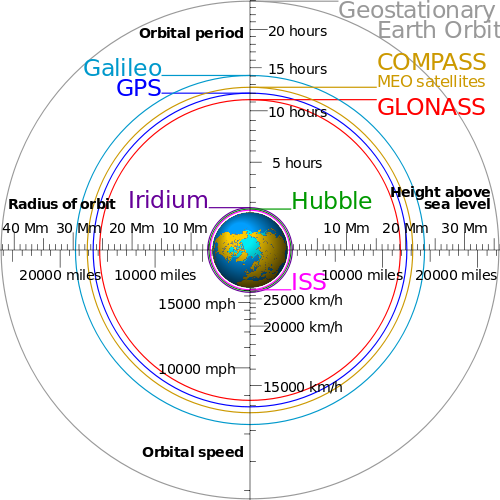
\includegraphics[width=45mm]{images/gnss_orbits.png}
\end{frame}

\begin{frame} \frametitle{GNSS Signals}
\begin{itemize}
	\item L1 (1.56542 GHz)/ L2(1.2276 GHz)
	\begin{itemize}
		\item C/A: (coarse acquisition) (1.023 million chips per second)
		\item P: pseudo-random sequence (10.23 million chips per second)
	\end{itemize}


	\item Navigation Message (Ephemeris)
	\begin{itemize}
		\item Takes 12.5 minutes to transfer full almanac
		\item Orbital parameters, and clock information
		\item Satellites calculate their own ephemeris every 2 hours
	\end{itemize}
\end{itemize}
\end{frame}

\begin{frame} \frametitle{Calculating Pseudorange}
\begin{itemize}
	\item Convolve segment of PRN with observed to find time message was sent
	\item start with C/A code to narrow in on P code
	\begin{itemize}
		\item P code is 26.716 TB long
		\item C/A code is 773,388 MB long
	\end{itemize}
	\item Recievers are rated on how many convolutions they can do per second
\end{itemize}
\centering
	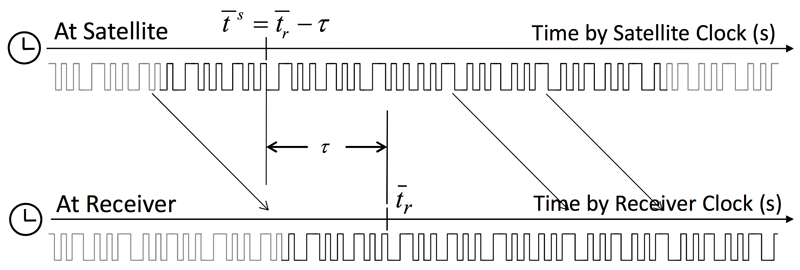
\includegraphics[width=45mm]{images/pseudorange_model.png}
\end{frame}

\begin{frame}\frametitle{Pseudorange Measurement}
Pseudorange is calculated from the time-of-flight of the signal from the satellite to the receiver
\begin{equation}
	\hat{\rho} = c\norm{\p_{s/e}^{e}\left(t_s\right)-\p_{b/e}^{e}\left(t_r\right)} + \delta^{atm} + c\left(\tau_{b}-\tau_{s}\right)+\xi_{\rho}
\end{equation}
where $t_s$ is the time the satellite sent the message, $t_r$ is the time of reception and $\tau_{b},\tau_{s}$ are the clock
bias of the receiver and satellite, respectively.
\end{frame}

\begin{frame}\frametitle{Effect of the Rotation of the Earth}
We have to account for the rotation of the earth when computing the relative distance between the satellite and receiver

\centering
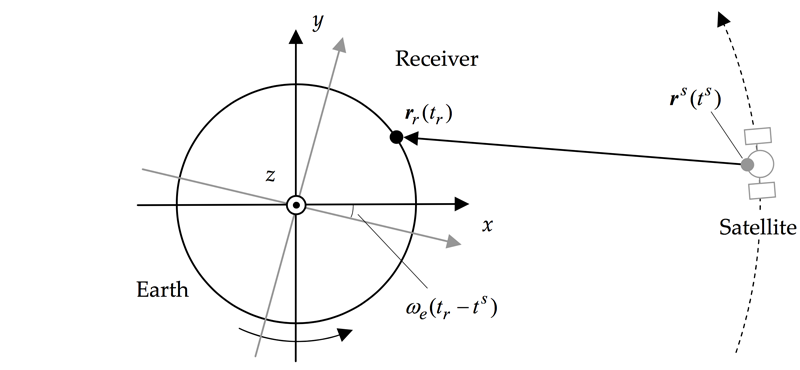
\includegraphics[width=70mm]{images/earth-rotation.png}
\end{frame}

\begin{frame}\frametitle{Pseudorange Measurement}
Here is the full pseudorange model put into terms of the recevier time (neglecting the Sagnac effect)
\begin{align*}
\hat{\rho}_{s}\left(\p_{s/e}^{e},\tau_{b},t_r\right) &= \norm{\p_{s/e}^{e}\left(t_r\right)-\p_{b/e}^{e}\left(t_r\right)}+\frac{1}{c}\w_{e}^{\top}
\skew{\p_{s/e}^{e}\left(t_r\right)}\p_{b/e}^{e}\left(t_r\right)\\
&+\delta^{atm}\left(\p_{s/e}^{e},\p_{b/e}^{e},t_r\right)+c\left(\tau_{b}-\tau_{s}\right)+\xi_{\rho}
\end{align*}
where $\delta^{atm}\left(\p_{s/e}^{e},\p_{b/e}^{e},t_r\right)$ is given
by the Klobuchar Algorithm and $\w_{e}$ is the rotation of the earth
% \centering
% 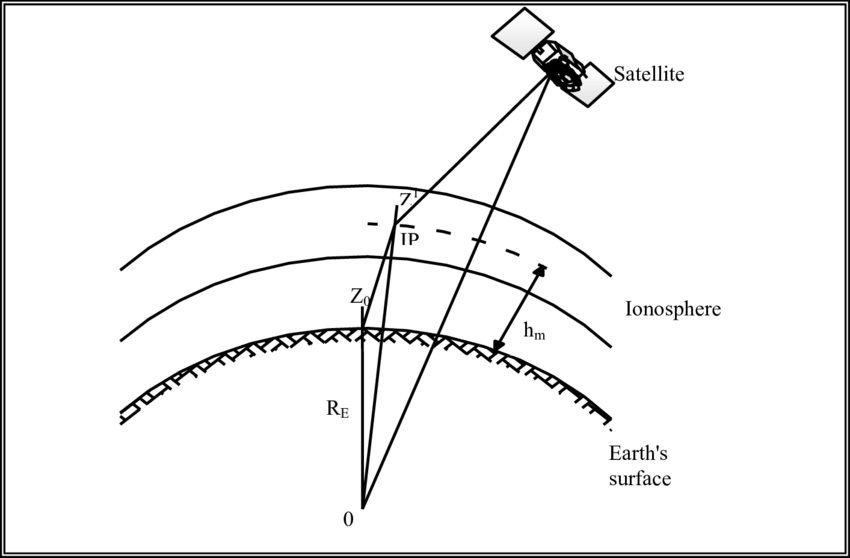
\includegraphics[width=45mm]{images/delays.png}
\end{frame}


\begin{frame}\frametitle{Pseudorange Rate}
\begin{itemize}
	\item Modern receivers are also able to measure the doppler on the P code signal.
	\item Doppler is not as affected by atmosphere
	\item $\dot{\rho}$ is more accurate than $\rho$
\end{itemize}
If we take the derivative of the pseudorange model, we get the pseudorange rate
\begin{equation}
	\dot{\hat{\rho}}_{s}\left(\p_{s/e}^{e},\tau_{b},t\right)\approx\norm{\dot{\p}_{s/e}^{e}\left(t\right)-\dot{\p}_{b/e}^{e}\left(t\right)}+c\left(\dot{\tau_{b}}-\dot{\tau}_{s}\right)+\xi_{\dot{\rho}}
\end{equation}
\end{frame}

\begin{frame}\frametitle{Calculating Position and Velocity Using $\rho$ and $\dot{\rho}$}
We wish to estimate the receiver position $\p^{r}$,
velocity $\v^{r}$, clock bias $\tau^{r}$ and clock bias rate $\dot{\tau}^{r}$
given the pseudorange and psuedorange rate measurement to $n$ satellites
$\prange_{i}$ and the satellite position.
\begin{equation}
	\x=\begin{bmatrix}\p& \v& \tau& \dot{\tau} \end{bmatrix}^\top,
\end{equation}
with measurements
\begin{equation}
	\z=\begin{bmatrix}\z^{0}& \vdots& \z^{n} \end{bmatrix}^\top, 
	\quad\z^{i}=\begin{bmatrix}\rho^{i}& \dot{\rho}^{i} \end{bmatrix}^\top.
\end{equation}
\end{frame}

\begin{frame}\frametitle{Calculating Position and Velocity Using $\rho$ and $\dot{\rho}$}
In other words, we wish to find $\x$ such that
\[
\z-\hat{\z}
\]
is minimized for all $n$ satellites, with

\begin{equation}
\hat{\z}=\begin{bmatrix}\begin{bmatrix}\norm{\x^{0}-\hat{\x}^{r}}+c\tau\\
\left(\v^{0}-\hat{\v}^{r}\right)^{\top}\hat{\e}^{0}+c\dot{\tau}
\end{bmatrix}\\
\vdots\\
\z^{n}
\end{bmatrix},\label{eq:pseudorange_opt}
\end{equation}
where
\[
\hat{\e}^{i}=\frac{\p^{i}-\hat{\p}^{r}}{\norm{\p^{i}-\hat{\p}^{r}}}.
\]
is the unit vector from the receiver to the satellite
\end{frame}

\begin{frame}\frametitle{Calculating Position and Velocity Using $\rho$ and $\dot{\rho}$}
Iterated approach:
\begin{enumerate}
	\item linearize our measurement model about some initial estimate
	\item calculate optimal step
	\item repeat until convergence
\end{enumerate}
\begin{align}
\begin{bmatrix}\delta\rho\\
\delta\dot{\rho}
\end{bmatrix} & =\begin{bmatrix}\rho^{i}-\rho{}_{0}^{i}\\
\dot{\rho}^{i}-\dot{\rho}{}_{0}^{i}
\end{bmatrix}\\
& =\begin{bmatrix}\norm{\p^{i}-\hat{\p}}-\norm{\p^{i}-\hat{\p}_{0}}+c\left(\hat{\tau}-\hat{\tau}_{0}\right)+\eta^{i}\\
\left(\v^{i}-\hat{\v}\right)^{\top}\hat{\e}^{i}-\left(\v^{i}-\hat{\v}_{0}^{r}\right)^{\top}\hat{\e}_{0}^{i}+c\left(\dot{\hat{\tau}}-\dot{\hat{\tau}}_{0}\right)
\end{bmatrix}\\
& \approx\begin{bmatrix}\norm{\p^{i}-\hat{\p}_{0}}-\frac{\p^{i}-\hat{\p_{0}}}{\norm{\p^{i}-\hat{\p}_{0}}}\tilde{\p}+c\tilde{\tau}-\norm{\p^{i}-\p_{0}}+\eta^{i}\\
\left(\v^{i}-\hat{\v}_{0}\right)^{\top}\hat{\e}_{0}^{i}+\tilde{\v}^{\top}\hat{\e}_{0}^{i}-\left(\v^{i}-\hat{\v}_{0}^{r}\right)^{\top}\e_{0}^{i}+c\left(\dot{\tilde{\tau}}\right)
\end{bmatrix}\\
& =\begin{bmatrix}-\left(\hat{\e}_{0}^{i}\right)^{\top} & 0 & c & 0\\
\tilde{\v}^{\top} & \hat{\e}_{0}^{i} & 0 & c
\end{bmatrix}\begin{bmatrix}\tilde{\p}\\
\tilde{\v}\\
\tilde{\tau}\\
\dot{\tilde{\tau}}
\end{bmatrix}+\begin{bmatrix}\eta^{i}\\
\dot{\eta}^{i}
\end{bmatrix}
\end{align}
\end{frame}


\begin{frame}\frametitle{Calculating Position and Velocity Using $\rho$ and $\dot{\rho}$}
Stack the linear equations for all $N$ satellites
\begin{align*}
\boldsymbol{\delta\prange}=\begin{bmatrix}\delta\prange^{1}\\
\delta\dot{\prange}^{1}\\
\vdots\\
\delta\prange^{N}\\
\delta\dot{\prange}^{N}
\end{bmatrix} & =\begin{bmatrix}-\left(\hat{\e}^{1}\right)^{\top} & 0 & c & 0\\
\tilde{\v}^{\top} & \hat{\e}^{1} & 0 & c\\
-\left(\hat{\e}^{2}\right)^{\top} & 0 & c & 0\\
\tilde{\v}^{\top} & \hat{\e}^{2} & 0 & c\\
\vdots\\
-\left(\hat{\e}^{N}\right)^{\top} & 0 & c & 0\\
\tilde{\v}^{\top} & \hat{\e}^{N} & 0 & c
\end{bmatrix}\begin{bmatrix}\tilde{\p}\\
\tilde{\v}\\
\tilde{\tau}\\
\dot{\tilde{\tau}}
\end{bmatrix}+\boldsymbol{\eta}\\
 & =G\begin{bmatrix}\tilde{\p}\\
\tilde{\v}\\
\tilde{\tau}\\
\dot{\tilde{\tau}}
\end{bmatrix}+\boldsymbol{\eta}
\end{align*}
\end{frame}


\begin{frame}\frametitle{Calculating Position and Velocity Using $\rho$ and $\dot{\rho}$}
Least-squares! 
\begin{align}
	\begin{bmatrix}\tilde{\p}\\
\tilde{\v}\\
\tilde{\tau}\\
\dot{\tilde{\tau}}
\end{bmatrix}&=\left(G^{\top}G\right)^{-1}G^{\top}\boldsymbol{\delta\rho}\\
\delta \x &= G^\dagger \left(\z - \hat{\z}\right) \\
{\x}^{+} &= {\x}^{-} + \delta{\x}
\end{align}
Repeat until convergence
\end{frame}

\begin{frame}\frametitle{Calculating Position and Velocity Using $\rho$ and $\dot{\rho}$}
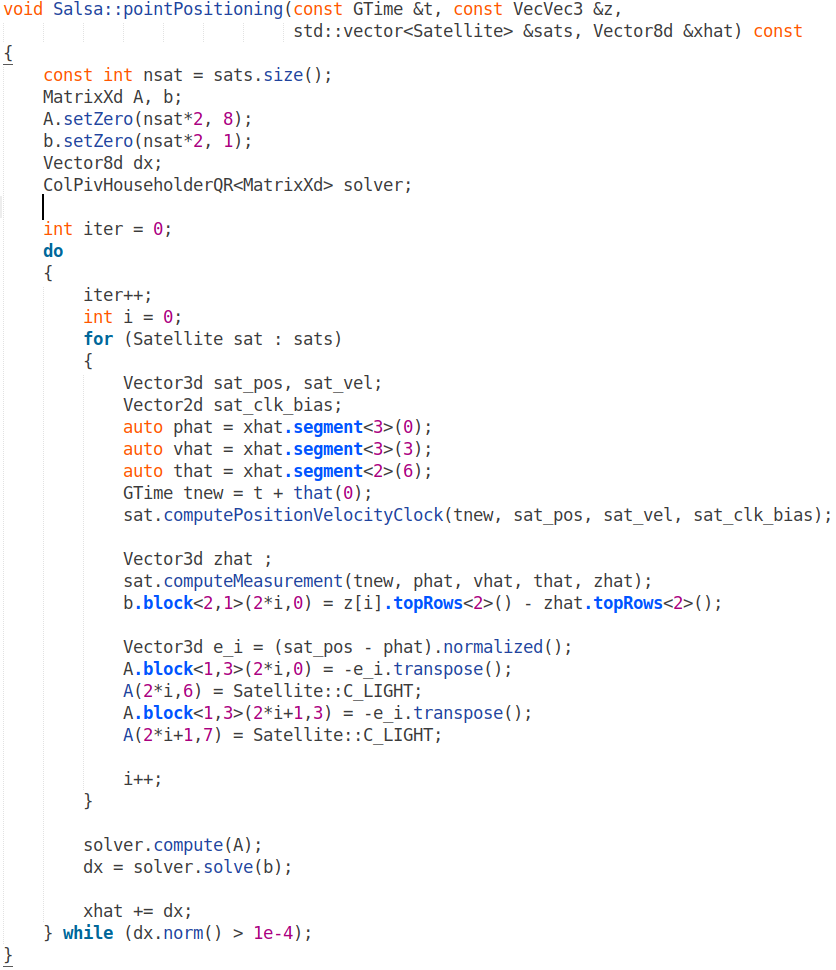
\includegraphics[height=0.8\textheight]{images/point_positioning_source_code.png}
\end{frame}

\begin{frame}\frametitle{Tightly-Coupled G-INS}
    Add the $\tau$ and $\dot{\tau}$ to the state of our usual EKF
    \begin{equation*}
    	\x = \begin{bmatrix} \p_{b/I}^I & \q_I^b & \v_{b/I}^b  & \beta_a & \beta_{\omega} & \tau & \dot{\tau} \end{bmatrix}
    \end{equation*}
    Where clock bias dynamics are
    \begin{equation*}
    	\dot{\x} = \begin{bmatrix} \vdots \\ \tau \\ \dot{\tau} \end{bmatrix} = \begin{bmatrix} \vdots \\ \dot{\tau} \\ \eta_\tau \end{bmatrix}
    \end{equation*}
    Fuse psuedorange directly as a measurement.

    Take care to handle the transform from the ECEF frame $e$ to the inertial frame $I$
\end{frame}

\begin{frame}\frametitle{Carrier-Phase Signal}
Modern receiver are also able to measure the number of cycles the carrier wave they are tracking have passed.

\begin{align}
\Phi_{b}^s&=\underbrace{\frac{c}{\lambda}\norm{\p_{i/e}^{e}-\p_{b/e}^{e}}}_{\text{range}}+\underbrace{\frac{c}{\lambda}\left(\tau_{b}-\tau_{i}\right)}_{\text{clk bias}}+\underbrace{\left(\Phi_{b,0}-\Phi_{i,0}+N_{b}^{s}\right)}_{\text{phase bias $B_{b}^{i}$}}+\frac{1}{\lambda}\left(T_b^i - I_b^s\right) + \xi_{\Phi} \\
&= \frac{1}{\lambda}\left( \rho_b^i + cd\tau_{b/i} + B_b^i + T_b^i - I_r^s \right) 
\end{align}

Where $\lambda$ is the wavelength, and $N_{b}^{s}$ is known as the \emph{integer ambiguity}.
\end{frame}

\begin{frame}\frametitle{Single Differencing}
We can cancel out the initial phase bias and the atmospheric error of the satellite by differencing carrier phase measurements between two receivers.
\begin{align*}
	\Phi_{rb}^{i} &=\Phi_{r}^{i}-\Phi_{b}^{i} \nonumber\\
	&= \frac{1}{\lambda}\left( \left(\rho_b^i + cd\tau_{b/i} + B_b^i + T_b^i - I_r^s\right)- \left(\rho_r^i + cd\tau_{r/i} + B_r^i + T_r^i - I_r^s \right)\right) \nonumber\\
	&= \frac{1}{\lambda} \left(\rho_{rb}^i -cd\tau_{rb}^i + B_{rb}^i\right)
\end{align*}
where
\begin{align*}
B_{rb}^{i} & =\left(\Phi_{r,0}-\Phi_{i,0}+N_{r}^{i}\right)-\left(\Phi_{b,0}-\Phi_{i,0}+N_{b}^{i}\right)\\
 & =\left(\Phi_{r,0}-\Phi_{b,0}+N_{rb}^{i}\right)
\end{align*}
\end{frame}

\begin{frame}\frametitle{Double Differencing}
Cancel out the clock error and the initial phase bias error
\begin{align*}
	\Phi_{rb}^{ij} &=\Phi_{rb}^{i}-\Phi_{rb}^{j} \nonumber\\
	&= \frac{1}{\lambda} \left(\left(\rho_{rb}^i -cd\tau_{rb}^i + B_{rb}^i\right) - \left(\rho_{rb}^j -cd\tau_{rb}^j + B_{rb}^j \right)\right)\\
	&= \frac{1}{\lambda} \left( \rho_{rb}^{ij} + N_{rb}^{ij} \right)
\end{align*}
because 
\begin{align*}
	d\tau_{rb}^{ij} &= \left( \left( \tau_r - \tau_i \right) - \right( \tau_b - \tau_i \left) \right) - \left( \left( \tau_r - \tau_j \right) - \right( \tau_b - \tau_j \left) \right) \\
	&= 0
\end{align*}
and
\begin{align*}
	B_{rb}^{ij} &= \left(\Phi_{r,0}-\Phi_{b,0}+N_{rb}^{i}\right) - \left(\Phi_{r,0}-\Phi_{b,0}+N_{rb}^{j}\right) \\
	&= N_{rb}^{ij} \in \mathbb{Z}
\end{align*}
\end{frame}

\begin{frame}\frametitle{Real-Time Kinematic GPS (RTK)}
   The goal of RTK is to estimate the position, velocity, clock bias of two GPS receivers.

   We use the fact that the integer ambiguities must be integers to acheive extremely high precision ($\pm$ 3cm) 
\begin{equation*}
   \x = \begin{bmatrix} \p_r & \p_b & \v_r & \v_b & \tau_r & \tau_b & \dot{\tau}_r & \dot{\tau}_b & N_{rb}^{ij}\end{bmatrix} ^\top 
\end{equation*}
with
\begin{equation*}
	\z^i = \begin{bmatrix} \rho_b^i & \dot{\rho}_b^i & \rho_r^i & \dot{\rho}_b^i & \Phi_r^i & \Phi_b^i \end{bmatrix} ^\top
\end{equation*}
\end{frame}

\begin{frame}\frametitle{Real-Time Kinematic GPS (RTK)}
This is a Mixed-Integer Programming (MIP) problem, and is typically implemented in a Kalman Filtering Framework.

Steps:
\begin{enumerate}
	\item acheive a floating-point estimate of $N_{rb}^{ij}$,
	\item perform a search across the likely region of integer combinations to get the most likely candidate.
	\item fuse best integer estimate into the Kalman Filter as a measurement.
\end{enumerate}
Doing this efficiently is a fertile research area. (I've never seen an MHE version, and it could probably be far superior, potentially even ``base-less'')
\end{frame}

\begin{frame}\frametitle{Real-Life RTK: Issues}
\begin{itemize}
	\item Getting estimates of the integer ambiguity is difficult.
	\item Losing lock with the satellite results in a \emph{cycle slip} - requires resolving for $N$
	\item Getting base data to the rover can often be a challenge
\end{itemize}
\end{frame}

\begin{frame}[t]\frametitle{Real-Life RTK: Solutions}    
\begin{itemize}
	\item Fixed-base
	\item Fixed-baseline
	\item Dual-frequency GNSS
\end{itemize}
	

\end{frame}







\end{document}


